\section{计算机学院本科生开题报告使用指南} \label{proposal}

本模板已经发布在 Overleaf 上,你可以打开直接使用(点击下图 \ref{overleaf-proposal} 所示中的 Open as Template)即可:

\begin{center}
  \color{ForestGreen}\href{https://www.overleaf.com/latex/templates/bei-jing-li-gong-da-xue-ben-ke-sheng-bi-ye-lun-wen-kai-ti-bao-gao-mo-ban/dgqdjptfqtrn}{https://www.overleaf.com/latex/templates/bei-jing-li-gong-da-xue-ben-ke-sheng-bi-ye-lun-wen-kai-ti-bao-gao-mo-ban/dgqdjptfqtrn}
\end{center}

\begin{figure}[H]
  \centering
  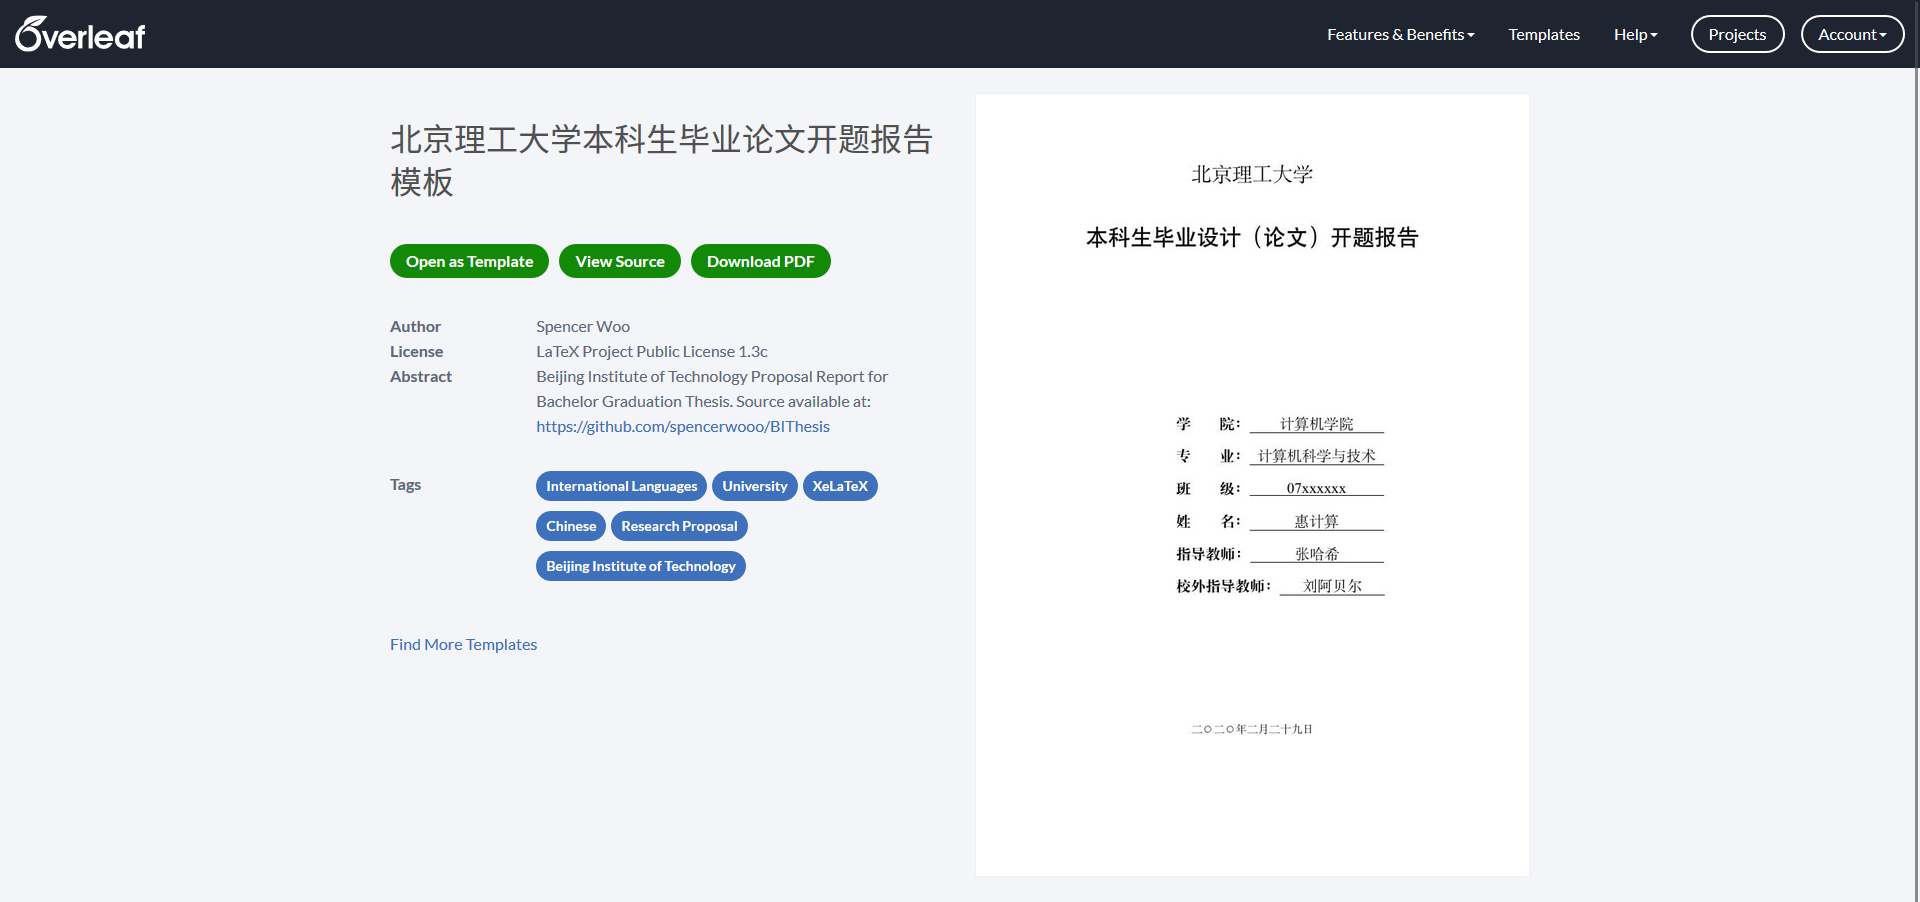
\includegraphics[width=\textwidth]{images/overleaf.png}
  \caption{Overleaf 在线版本的开题报告模板}
  \label{overleaf-proposal}
\end{figure}

Overleaf 缺少一些微软版权字体(比如宋体、黑体等),\textbf{因此如果你希望格式完全准确,请使用本机进行编辑。}

\subsection{熟悉项目}
% 输出文件数,第一行百分号 % 不能删,详见:http://tug.ctan.org/macros/generic/dirtree/dirtree.pdf
\dirtree{%
.1 /.
.2 README.md.
.2 main.pdf.
.2 main.tex.
.2 merge-sort-recursion-tree.png.
.2 misc.
.3 cover.tex.
.3 refs.bib.
.3 reviewTableBlank.pdf.
}

本项目由四个主要文件编译而成:\texttt{main.tex}、\texttt{cover.tex}、\texttt{refs.bib} 与\\ \texttt{reviewTableBlank.pdf}(也包括文档中所涉及到的图片等素材文件,比如:\\ \texttt{merge-sort-recursion-tree.png})。请大家重点关注这四个文件的功能与作用:

\begin{itemize}
  \item[\color{RubineRed}\textbf{\texttt{main.tex}}] 开题报告的开始文件(主文件),你的报告内容应该从此文件开始撰写。\texttt{main.tex} 中有详细的注释,介绍了每一部分内容都有什么作用,请仔细阅读后进行相应的修改、
  \item[\color{RubineRed}\textbf{\texttt{main.pdf}}] 开题报告编译得到的 PDF 文件
  \item[\color{RubineRed}\textbf{\texttt{./misc}}] 开题报告中所需要的杂项所在文件夹,其中包含有:
  \begin{itemize}
    \item[\color{RoyalBlue}\texttt{cover.tex}] 开题报告封面,按照教务部提供的封面设计,如无特殊需要请不要修改
    \item[\color{RoyalBlue}\texttt{reviewTableBlank.pdf}] 开题报告 PDF 格式的“评审表”,由于考虑到评审表后期由评委老师填写,因此本部分如无需要也无需改动
    \item[\color{RoyalBlue}\texttt{refs.bib}] 开题报告的参考文献 {\hologo{BibTeX}} 数据库,你应该向其中加入开题报告中所需要的所有参考文献的 {\hologo{BibTeX}} 格式引用(详见下文)
  \end{itemize}
\end{itemize}

\subsection{你的内容从哪里开始?}
开题报告项目结构相对来说比较简单,因此你只需要重点关注 \texttt{main.tex} 这一文件 —— 项目的主文件。你的内容应该从 \texttt{main.tex} 第 127 行 的 \texttt{\%内容开始} 开始。你需要重点关注的部分有:

\begin{table}[H]
\centering
\caption{开题报告内容概要}
\label{tab:proposalreport}
\resizebox{\textwidth}{!}{%
\begin{tabular}{@{}rll@{}}
\toprule
\textbf{文章部分} & \textbf{内容主旨}      & \textbf{对应 {\LaTeX} 模板 section}    \\ \midrule
第一部分 & 选题内容      & \texttt{\textbackslash{}section\{毕业设计(论文)\}}        \\ \midrule
第二部分 & 研究方案      & \texttt{\textbackslash{}section\{研究方案\}}            \\ \midrule
2-1  & 主要任务      & \texttt{\textbackslash{}subsection\{本选题的主要任务\}}     \\
2-2  & 技术方案      & \texttt{\textbackslash{}subsection\{技术方案的分析、选择\}}   \\
2-3  & 实施方案所需环境  & \texttt{\textbackslash{}subsection\{实施技术方案所需的条件\}}  \\
2-4  & 存在问题与技术关键 & \texttt{\textbackslash{}subsection\{存在的主要问题和技术关键\}} \\
2-5  & 预期研究目标    & \texttt{\textbackslash{}subsection\{预期能够达到的研究目标\}}  \\ \midrule
第三部分 & 课题计划进度表   & \texttt{\textbackslash{}section\{课题计划进度表\}}         \\ \bottomrule
\end{tabular}%
}
\end{table}

以及最后的“参考文献”。你应该将参考文献的 {\hologo{BibTeX}} 引用复制进入 \texttt{./misc/refs.bib},并在正文中用 \verb|\cite{}| 的方法进行引用。其中 {\hologo{BibTeX}} 格式的引用内容可以在谷歌学术中搜索文章直接复制得到,也可以考虑使用 Zotero 等文献管理工具批量生成。

\subsection{其他注意事项}
\tipbox{有关具体的 {\LaTeX} 语法,请参考前文中《第二章 \ref{subsec:latex-grammar}》给出的参考链接与学习文档。以下是模板中提供的一些示例性代码。}

\subsubsection{插入图片}
如果你希望加入图片,可以将图片直接放在根目录(比如此处的\\ \texttt{merge-sort-recursion-tree.png}),或者统一将图片安置在一个文件夹下,在正文里按照相对路径进行引用。模板中有一处插入图片的参考样例,位于 \texttt{main.tex} 的 \href{https://github.com/spencerwooo/BIThesis/blob/master/proposal-report/main.tex#L138}{第 138 行},可以进行参考。比如,我填入一个放在 \texttt{images/BIT\_Name.jpg} 处的图片:

\begin{minted}[frame=single,linenos,breaklines]{latex}
  \begin{figure}[!ht]
    \centering
    
\includegraphics[width=0.6\linewidth]{images/BIT_Name.jpg}
    \caption{北京理工大学(一张示意图)}
    \label{fig:BITName}
  \end{figure}
\end{minted}

这样就会渲染如图 \ref{fig:BITName} 的效果:

\begin{figure}[!ht]
  \centering
  
\includegraphics[width=0.6\linewidth]{images/BIT_Name.jpg}
  \caption{北京理工大学(一张示意图)}
  \label{fig:BITName}
\end{figure}

\subsubsection{插入表格}
如果你希望插入表格,可以统一使用 \href{https://www.tablesgenerator.com/}{LaTeX Tables Generator} 进行生成,再粘贴进入模板之中。模板中有两处表格的参考样例,分别位于 \href{https://github.com/spencerwooo/BIThesis/blob/master/proposal-report/main.tex#L151}{第 151 行} 和 \href{https://github.com/spencerwooo/BIThesis/blob/master/proposal-report/main.tex#L176}{第 176 行},可以进行参考。比如:

\begin{minted}[frame=single,linenos,breaklines]{latex}
  \begin{table}[!ht]
    \centering
    \caption{硬件、软件环境}
    \label{tab:soft-hardware}
    \begin{tabular}{@{}lcl@{}}
      \toprule
                                & 指标     & \multicolumn{1}{c}{版本参数} \\ \midrule
      \multirow{2}{*}{硬件环境} & CPU      & Intel i7-6500U               \\ \cmidrule(l){2-3}
                                & RAM      & 8 GB                         \\ \midrule
      \multirow{2}{*}{软件环境} & 操作系统 & \begin{tabular}[c]{@{}l@{}}Windows 10 Pro x86\_64\\  Ubuntu 18.04.3 LTS\end{tabular}    \\ \cmidrule(l){2-3}
                                & Python   & Python 3.7.6                 \\ \bottomrule
    \end{tabular}
  \end{table}
\end{minted}

渲染效果如表 \ref{tab:proposalreport} 所示:

\begin{table}[!ht]
  \centering
  \caption{硬件、软件环境}
  \label{tab:soft-hardware}
  \begin{tabular}{@{}lcl@{}}
    \toprule
                              & 指标     & \multicolumn{1}{c}{版本参数} \\ \midrule
    \multirow{2}{*}{硬件环境} & CPU      & Intel i7-6500U               \\ \cmidrule(l){2-3}
                              & RAM      & 8 GB                         \\ \midrule
    \multirow{2}{*}{软件环境} & 操作系统 & \begin{tabular}[c]{@{}l@{}}Windows 10 Pro x86\_64\\  Ubuntu 18.04.3 LTS\end{tabular}    \\ \cmidrule(l){2-3}
                              & Python   & Python 3.7.6                 \\ \bottomrule
  \end{tabular}
\end{table}
